\section{Data and data contracts}\label{sec:data}

\subsection{Sources}\label{sec:data-sources}

Four data sources enter the product; a fifth, the sector statistics of the introduction, is context and enters no
computation.

\emph{The ten HP500 surveys.} Table A1 of Rocha, Campos, Silva and Tavares~\cite{rocha2024} (Minerals, MDPI, open access
under CC BY 4.0, \url{https://doi.org/10.3390/min14090919}) gives, for ten surveys of a Metso HP500 secondary cone crusher at
an itabirite iron-ore operation, the closed-side setting, the feed $80\%$ passing size $f_{80}$, the solid feed rate and the
motor power estimated from the measured current. The paper states that the ten surveys were carried out over three years
of operation of the secondary crushing stage of the Minas Rio plant, which runs four HP500 crushers in parallel in closed
circuit with $25$~mm screens, all designed with a nominal setting of $38$~mm, an installed power of $355$~kW and a medium
cavity, and that the surveys were taken with the crushers operating with a full chamber; it gives no date per survey. Its
model is an Andersen-Whiten crusher model implemented in the Integrated Extraction Simulator, with a separate empirical
model of the maximum throughput (Section~\ref{sec:m-hp500}). The table is transcribed into \texttt{data/\allowbreak{}examples/\allowbreak{}hp500-surveys.csv}
(ten rows, five columns, $210$~bytes) and validated by the \texttt{hp500-survey} contract below. Table~\ref{tab:surveys}
lists the ten rows beside the calibrated engine's outputs at each of them. Across the surveys the setting spans $38$ to
$55$~mm, the feed $f_{80}$ $47$ to $140$~mm, the feed rate $813$ to $1639$~t/h and the power $187$ to $355$~kW. The measured
power is correlated with the setting ($r=-0.82$) and with the feed rate ($r=-0.85$), and the feed rate with the setting
($r=+0.81$), so a tighter setting draws more power at a lower feed rate (Figure~\ref{fig:surveys}). The paper prints the
product size distributions only as figures, so no product size is measured in the product's data.

\emph{The circuit cases.} The seventeen circuit cases are the product's own table \texttt{data/\allowbreak{}examples/\allowbreak{}params.csv} (MIT
licence, seventeen rows and nine columns, one operating point each): two gyratory, two jaw, six secondary cone, two tertiary
cone and two short-head cases, and three controls, a pass-through case (CP1, a setting of $160$~mm against a feed $F_{80}$ of
$126$~mm), an invalid case (CI1, a setting of $280$~mm, above the top size of the grid) and a synthetic anchor (CK1). The case
CK1 is synthetic because the only other open industrial cone calibration found, Duarte et al.~\cite{duarte2021}, reports
seven operating points of an HP400 and a CH660 with the setting, the throughput and the feed $F_{80}$ only, without throw,
speed, ore properties or power, and with its size data as plots. Table~\ref{tab:cases} lists the $27$ cases as baked.

\emph{The engine sweeps of the learned models.} The training data of the surrogate and the autoencoder are generated, not
measured: a Latin-hypercube sweep of the canonical engine, $1400$ points per machine class over that class's own ranges
(Table~\ref{tab:machines}), labelled by the engine, with degenerate draws dropped (a setting at or above the feed top size, an
ill-conditioned matrix, a reduction ratio below $1.02$ or a non-positive $P_{80}$), which leaves $6430$ training points. An
independent second draw with another seed ($67890$, $480$ points per class) leaves $2196$ held-out points.

\emph{Vendor bounds.} Two sourced warnings of the engine read published vendor documents: the minimum closed-side setting of
the HP Series standard ($16$~mm) and short-head ($6$~mm) chambers and the typical reduction ratios of $3$ to $5$ and $2$ to
$4$ from the Metso HP wear-parts application guide~\cite{metsoHP}; the smallest minimum setting of the Nordberg C Series jaw
crushers ($40$~mm, the C80)~\cite{metsoC}; and the reduction ratio of $3$ to $4$ for jaw and gyratory crushers from the Metso
handbook~\cite{metsoBasics}. No vendor minimum setting was found for a primary gyratory, so that check is skipped.

\emph{The splits and why.} The circuit cases are not fitted and need no split. The ten surveys are too few for a held-out
block, so every fitted quantity is evaluated by leave-one-survey-out: ten folds of nine training surveys and one held-out
survey, the same folds for every predictor (Section~\ref{sec:m-crushercal}). The learned models are judged on an independent
draw rather than a split of the training draw, so that a point near a training point does not flatter the error.

\begin{table}[!t]
\centering
\caption{The ten HP500 surveys of Rocha et al.~\cite{rocha2024} as committed, with the calibrated engine evaluated at each
measured setting and feed $f_{80}$ (throw $34$~mm, speed $360$~rpm): its grid $F_{80}$, product $P_{80}$, throughput $Q$, Bond
draw and the published current-based power $1.30\,P_d+110$. Generated from \texttt{backbone.json}.}
\label{tab:surveys}
\footnotesize
% generated by figures/make_tables.py; do not edit by hand
\begin{tabular}{@{}r rrrr rrrrr@{}}
\toprule
 & \multicolumn{4}{c}{Measured (Table A1)} & \multicolumn{5}{c}{Calibrated engine} \\ \cmidrule(lr){2-5}\cmidrule(lr){6-10}
Survey & CSS (mm) & $f_{80}$ (mm) & Feed (t/h) & Power (kW) & $F_{80}$ (mm) & $P_{80}$ (mm) & $Q$ (t/h) & Bond (kW) & $P_c$ (kW) \\
\midrule
1 & $54$ & $88$ & $1639$ & $209$ & $84.86$ & $32.56$ & $1208.9$ & $229.5$ & $408.3$ \\
2 & $54$ & $84$ & $1267$ & $212$ & $81.70$ & $31.36$ & $1208.9$ & $233.7$ & $413.9$ \\
3 & $48$ & $47$ & $1240$ & $262$ & $47.15$ & $21.23$ & $1106.7$ & $224.9$ & $402.3$ \\
4 & $48$ & $88$ & $1034$ & $349$ & $84.86$ & $30.80$ & $1106.7$ & $225.7$ & $403.4$ \\
5 & $48$ & $62$ & $1124$ & $325$ & $61.66$ & $24.54$ & $1106.7$ & $234.8$ & $415.2$ \\
6 & $40$ & $79$ & $813$ & $355$ & $77.55$ & $26.54$ & $970.5$ & $222.5$ & $399.3$ \\
7 & $38$ & $140$ & $1050$ & $306$ & $118.94$ & $36.60$ & $936.5$ & $196.1$ & $365.0$ \\
8 & $44$ & $123$ & $1138$ & $325$ & $109.85$ & $35.69$ & $1038.6$ & $212.7$ & $386.6$ \\
9 & $40$ & $81$ & $820$ & $350$ & $79.24$ & $26.97$ & $970.5$ & $221.6$ & $398.0$ \\
10 & $55$ & $81$ & $1334$ & $187$ & $79.24$ & $30.72$ & $1225.9$ & $237.5$ & $418.7$ \\
\bottomrule
\end{tabular}

\end{table}

\begin{figure}[!t]
\centering
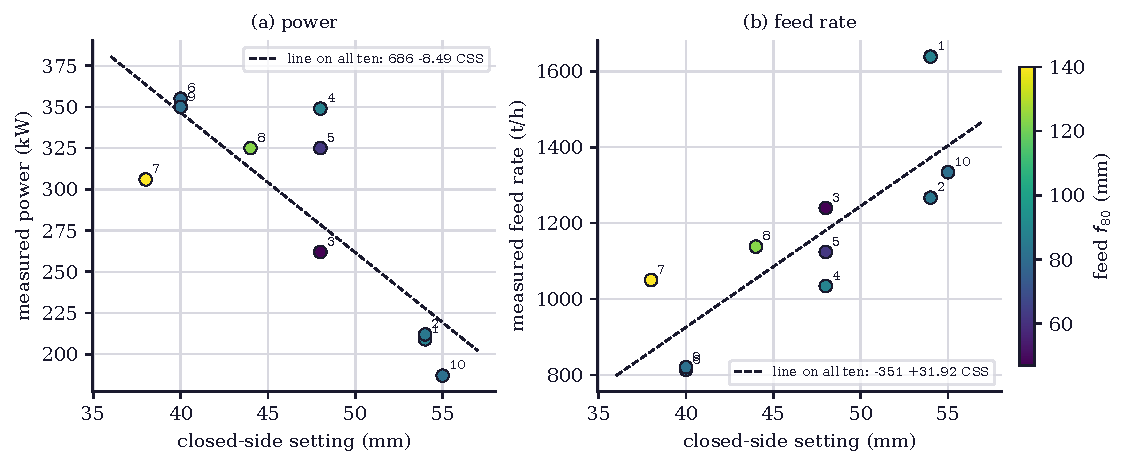
\includegraphics[width=\textwidth]{fig-surveys.pdf}
\caption{The ten HP500 surveys: (a) measured motor power and (b) measured feed rate against the closed-side setting, coloured
by the measured feed $f_{80}$ and numbered as in the published table, with the least-squares line on the setting fitted to all
ten surveys.}
\label{fig:surveys}
\end{figure}

\begin{table}[!t]
\centering
\caption{The $27$ baked cases, from their manifests and traces: machine, setting, throw and speed, the engine's feed $F_{80}$,
product $P_{80}$, reduction ratio, throughput, power, regime and validity. The ten HP500 cases run on the calibrated lane.}
\label{tab:cases}
\scriptsize
% generated by figures/make_tables.py; do not edit by hand
\begin{tabular}{@{}l l rrr rrr rr l l@{}}
\toprule
Case & Machine & CSS & Throw & Speed & $F_{80}$ & $P_{80}$ & $F_{80}/P_{80}$ & $Q$ & Power & Regime & Valid \\
\multicolumn{1}{c}{} &  & (mm) & (mm) & (rpm) & (mm) & (mm) &  & (t/h) & (kW) &  &  \\
\midrule
CI1 & secondary cone & $280$ & $30$ & $360$ & $126.0$ & $126.0$ & $1.00$ & $4037$ & $0$ & invalid & no \\
CK1 & secondary cone & $25$ & $30$ & $350$ & $116.2$ & $21.7$ & $5.35$ & $547$ & $316$ & choke & yes \\
CP1 & secondary cone & $160$ & $30$ & $360$ & $126.0$ & $112.3$ & $1.12$ & $2395$ & $56$ & pass-through & no \\
G01 & gyratory & $165$ & $30$ & $150$ & $180.3$ & $153.6$ & $1.17$ & $4629$ & $145$ & choke & yes \\
G02 & gyratory & $195$ & $32$ & $160$ & $185.8$ & $170.1$ & $1.09$ & $5414$ & $68$ & pass-through & no \\
H01 & short-head cone & $6$ & $14$ & $500$ & $29.8$ & $4.6$ & $6.55$ & $216$ & $273$ & choke & yes \\
H02 & short-head cone & $10$ & $16$ & $470$ & $41.6$ & $8.6$ & $4.86$ & $300$ & $319$ & choke & yes \\
HP500-01 & secondary cone & $54$ & $34$ & $360$ & $84.9$ & $32.6$ & $2.61$ & $1209$ & $408$ & choke & yes \\
HP500-02 & secondary cone & $54$ & $34$ & $360$ & $81.7$ & $31.4$ & $2.61$ & $1209$ & $414$ & choke & yes \\
HP500-03 & secondary cone & $48$ & $34$ & $360$ & $47.1$ & $21.2$ & $2.22$ & $1107$ & $402$ & pass-through & no \\
HP500-04 & secondary cone & $48$ & $34$ & $360$ & $84.9$ & $30.8$ & $2.76$ & $1107$ & $403$ & choke & yes \\
HP500-05 & secondary cone & $48$ & $34$ & $360$ & $61.7$ & $24.5$ & $2.51$ & $1107$ & $415$ & choke & yes \\
HP500-06 & secondary cone & $40$ & $34$ & $360$ & $77.6$ & $26.5$ & $2.92$ & $970$ & $399$ & choke & yes \\
HP500-07 & secondary cone & $38$ & $34$ & $360$ & $118.9$ & $36.6$ & $3.25$ & $936$ & $365$ & choke & yes \\
HP500-08 & secondary cone & $44$ & $34$ & $360$ & $109.9$ & $35.7$ & $3.08$ & $1039$ & $387$ & choke & yes \\
HP500-09 & secondary cone & $40$ & $34$ & $360$ & $79.2$ & $27.0$ & $2.94$ & $970$ & $398$ & choke & yes \\
HP500-10 & secondary cone & $55$ & $34$ & $360$ & $79.2$ & $30.7$ & $2.58$ & $1226$ & $419$ & choke & yes \\
J01 & jaw & $125$ & $40$ & $300$ & $182.9$ & $126.4$ & $1.45$ & $923$ & $70$ & choke & yes \\
J02 & jaw & $80$ & $36$ & $280$ & $184.2$ & $82.4$ & $2.24$ & $622$ & $100$ & choke & yes \\
S01 & secondary cone & $32$ & $30$ & $360$ & $126.0$ & $27.7$ & $4.55$ & $643$ & $287$ & choke & yes \\
S02 & secondary cone & $40$ & $32$ & $300$ & $147.1$ & $33.8$ & $4.35$ & $754$ & $235$ & choke & yes \\
S03 & secondary cone & $50$ & $30$ & $470$ & $152.0$ & $42.3$ & $3.59$ & $856$ & $334$ & choke & yes \\
S04 & secondary cone & $80$ & $36$ & $360$ & $161.8$ & $70.5$ & $2.30$ & $1341$ & $275$ & choke & yes \\
S05 & secondary cone & $16$ & $26$ & $360$ & $75.2$ & $13.6$ & $5.51$ & $397$ & $273$ & choke & yes \\
S06 & secondary cone & $12$ & $22$ & $360$ & $88.7$ & $9.1$ & $9.80$ & $315$ & $315$ & choke & yes \\
T01 & tertiary cone & $8$ & $16$ & $400$ & $39.0$ & $7.1$ & $5.48$ & $240$ & $228$ & choke & yes \\
T02 & tertiary cone & $10$ & $18$ & $410$ & $45.0$ & $9.6$ & $4.67$ & $285$ & $281$ & choke & yes \\
\bottomrule
\end{tabular}

\end{table}

\subsection{The contract catalog}\label{sec:data-catalog}

Every boundary between two components of the product is a data contract: one JSON Schema file (or, for the interface, one
OpenAPI document), an example, a test on the producer side and a test on the consumer side, a stated behaviour when the data
are missing, and a version that moves by semantic versioning with the schema. The catalog
\texttt{docs/\allowbreak{}contracts/\allowbreak{}catalog.md} lists \ncontracts{} contracts (Table~\ref{tab:contracts}); the TypeScript types of the web are
generated from the same schema files, so a change to a contract fails the web build until both sides follow it. Missing data
are described by one vocabulary of states: \emph{available}, \emph{missing} (the document is absent), \emph{partial} (some
files a document names are absent), \emph{stale} (the document was baked by an older version of the product), \emph{training}
(a model bundle is absent or fails its checksum, so the slot answers with its baseline) and \emph{provider} (a stand-in serves
the contract). The readiness document records the state of every contract for one build, and every view of the web shows it.
The subsections below describe each contract; the field tables generated from the schema files are in
Appendix~\ref{app:schemas}.

\begin{table}[!t]
\centering
\caption{The \ncontracts{} data contracts of the product, generated from the catalog: identifier, version, producing module,
schema file and status in the committed build. Their fields are listed in Appendix~\ref{app:schemas}.}
\label{tab:contracts}
\footnotesize
% generated by figures/make_tables.py; do not edit by hand
\begin{tabular}{@{}l l p{0.29\textwidth} p{0.30\textwidth} l@{}}
\toprule
Contract & Version & Producer (owner) & Schema file & Status \\
\midrule
\texttt{params-record} & 1.0.1 & \texttt{pipeline/io/contract.py} & \texttt{params-record.schema.json} & real \\
\texttt{hp500-survey} & 1.0.1 & \texttt{pipeline/hp500/surveys.py} & \texttt{hp500-survey.schema.json} & real \\
\texttt{case-index} & 1.0.1 & \texttt{pipeline/core/manifest.py} & \texttt{case-index.schema.json} & real \\
\texttt{case-manifest} & 1.1.1 & \texttt{pipeline/core/manifest.py} & \texttt{case-manifest.schema.json} & real \\
\texttt{trace} & 1.0.2 & \texttt{pipeline/core/trace.py} & \texttt{trace.schema.json} & real \\
\texttt{hp500-backbone} & 1.0.1 & \texttt{pipeline/hp500/backbone.py} & \texttt{hp500-backbone.schema.json} & real \\
\texttt{hp500-loo} & 1.2.1 & \texttt{pipeline/hp500/loo.py} & \texttt{hp500-loo.schema.json} & real \\
\texttt{hp500-crusherbayes} & 1.0.1 & \texttt{pipeline/hp500/crusherbayes.py} & \texttt{hp500-crusherbayes.schema.json} & real \\
\texttt{hp500-comparison} & 1.0.1 & \texttt{pipeline/hp500/comparison.py} & \texttt{hp500-comparison.schema.json} & real \\
\texttt{surrogate-model} & 1.0.1 & \texttt{pipeline/stages/train.py} & \texttt{surrogate-model.schema.json} & real \\
\texttt{anomaly-model} & 1.0.1 & \texttt{pipeline/stages/train.py} & \texttt{anomaly-model.schema.json} & real \\
\texttt{model-metrics} & 1.0.1 & \texttt{pipeline/stages/evaluate.py} & \texttt{model-metrics.schema.json} & real \\
\texttt{readiness} & 1.0.1 & \texttt{pipeline/core/readiness.py} & \texttt{readiness.schema.json} & real \\
\texttt{api} & 1.0.1 & \texttt{app/} & \texttt{api.openapi.json} & real \\
\bottomrule
\end{tabular}

\end{table}

\subsection{params-record: one operating point}\label{sec:data-params}

The \texttt{params-record} contract (version \cver{params-record}, fields in Table~\ref{tab:schema-params-record}, schema \texttt{params-record.schema.json}) is the ingestion contract of
the circuit cases: one row of \texttt{params.csv} as \texttt{pipeline/\allowbreak{}io/\allowbreak{}contract.py} accepts it. Its nine required fields
are the case identifier (string, pattern of one capital letter followed by one to fifteen capitals, digits or hyphens), the
machine class (one of five values), the closed-side setting \texttt{css\_mm} (number, above $0$ and at most $600$~mm), the
throw \texttt{throw\_mm} ($1$ to $100$~mm), the speed \texttt{speed\_rpm} ($50$ to $1000$~rpm), the feed characteristic size
\texttt{feed\_x63\_mm} (above $0$ and at most $2000$~mm), the uniformity exponent \texttt{feed\_m} ($0.3$ to $4$), the ore
competence \texttt{ore\_axb} ($10$ to $1000$) and the Bond work index \texttt{ore\_wi} ($2$ to $40$~kWh/t). A value is parsed,
never coerced: a row the schema refuses is rejected with its reason, and a physically unusual but valid row (a setting at or
above the feed's $F_{80}$ or its top size) is accepted and flagged with the engine's own codes, so the controls are baked and
shown. The consumers are the bake (\texttt{pipeline/\allowbreak{}pipeline.py}) and the tests of both sides. Missing-data behaviour: a
rejected row is dropped with its reason and the bake goes on with the accepted rows, while readiness lists the rejected case
identifiers as \emph{partial}; with no source table at all, readiness says \emph{missing} and the bake uses the registry's
cases.

\subsection{hp500-survey: one measured survey}\label{sec:data-survey}

The \texttt{hp500-survey} contract (version \cver{hp500-survey}, fields in Table~\ref{tab:schema-hp500-survey}) is the ingestion contract of the real data: one row of
\texttt{hp500-surveys.csv} as \texttt{pipeline/\allowbreak{}hp500/\allowbreak{}surveys.py} accepts it. Its five required fields are the survey number
(integer, $1$ to $10$, consecutive without a gap), the measured feed $f_{80}$ (number, above $0$ and at most $400$~mm), the
measured closed-side setting (above $0$ and at most $200$~mm), the measured solid feed rate \texttt{feed\_tph} (above $0$ and at
most $5000$~t/h) and the crusher power estimated from the measured current \texttt{power\_kw} (above $0$ and at most
$1000$~kW). The bounds are wide on purpose: they refuse a unit error, such as a power in watts, and a typing error, not a
plausible survey. The producer is the transcription of Table A1, its consumers the HP500 cases, the backbone, CrusherCal and
CrusherBayes. An acceptance rule of the product applies to this contract alone: if a re-transcription of the published table
disagrees with the committed file, the real lane is removed from the build until the table is corrected. Missing-data behaviour: with no
survey table, readiness says \emph{missing}, the bake skips the ten real cases and the four HP500 documents, the case selector
lists no real survey, and the survey views of the web say that the data are not available with the reason; a rejected row is
dropped with its reason, its case is not baked and readiness lists the survey number as \emph{partial}.

\subsection{case-index: the inventory of a bake}\label{sec:data-index}

The \texttt{case-index} contract (version \cver{case-index}, fields in Table~\ref{tab:schema-case-index}, \texttt{data/\allowbreak{}derived/\allowbreak{}manifests/\allowbreak{}index.json}, schema
\texttt{chancadem.index/\allowbreak{}v1}) is the flat inventory the web reads first. It carries the product version that baked it
(\texttt{engine\_version}, pattern \texttt{X.XX.XXX}), the number of cases (integer, at least one; $27$ in the committed build),
the default case (\texttt{S01}), one entry per case with its identifier, its title and category in English and Spanish, whether
it is real or synthetic and the relative path of its manifest, and the list of the further files the site serves: the five
model files, the four HP500 documents and the model metrics. Rules the schema cannot state are checked by the tests: the count
equals the number of entries, every path exists, and the default case is listed. It is produced by
\texttt{pipeline/\allowbreak{}core/\allowbreak{}manifest.py} (\texttt{build\_index}) and read by the web's case selector, the copy step of the site build
(which copies exactly the files the index declares) and the dormant interface. Missing-data behaviour: without an index the site
build stops at its copy step, because a site without an inventory would show nothing reliably; the interface answers $503$ with
the state \emph{missing}. When \texttt{engine\_version} is older than the product version, readiness says \emph{stale} with both
versions and the views show it.

\subsection{case-manifest: one baked case}\label{sec:data-manifest}

The \texttt{case-manifest} contract (version \cver{case-manifest}, fields in Table~\ref{tab:schema-case-manifest}, one file \texttt{data/\allowbreak{}derived/\allowbreak{}manifests/\allowbreak{}<case>.json} per case, schema
\texttt{chancadem.manifest/\allowbreak{}v1}) is the authoritative record of one case and a pure function of its parameters and seed: it
holds no wall-clock time, so a re-bake does not change it. Its twenty required fields include the case identifier, the
bilingual title, category and expected band in words, the circuit stage (primary, secondary, tertiary or control), the kind of
control (none, negative, invalid or calibration), the case context (the question, the variables and how to read the views),
the engine package and version, the operating point exactly as the ingestion contract accepted it with the \texttt{calibrated}
switch, the seed, the artifact (relative path, format, trace schema, size in bytes and SHA-256), the lane decision of the lane
check (live or precompute, with the measured trace size and the budgets of $1500$~ms and $256$~KiB), the flags as stable codes,
the result metrics, which model answered per model slot (the released model or its baseline), the expected range of each
metric, and the source. A real case adds the survey row as measured; its metrics add the signed percentage error of the
throughput and the power against the measured values ($-10.75\%$ and $+53.55\%$ for survey 3). The producer is
\texttt{pipeline/\allowbreak{}core/\allowbreak{}manifest.py}; the consumers are the web workbench and the interface. Missing-data behaviour: a manifest the
index lists but that is absent is reported by readiness as \emph{partial} with its path, the selector marks that case as not
available and the other cases work, and the interface answers $404$ for it; staleness follows the index.

\subsection{trace: the replay artifact}\label{sec:data-trace}

The \texttt{trace} contract (version \cver{trace}, fields in Table~\ref{tab:schema-trace}, \texttt{data/\allowbreak{}derived/\allowbreak{}<case>/\allowbreak{}trace.json}, schema \texttt{chancadem.trace/\allowbreak{}v1}) holds
what the engine computed at the operating point of a case: the $29$ sieve edges and $28$ mid-sizes in millimetres, the feed
and product cumulative passing at each edge and mass per class (fractions in $[0,1]$), the classification $C(d)$ at each
mid-size, the $t_{10}$ of the appearance function as a fraction in $[0, 0.44]$ ($0.364$ for S01; the schema keeps the upper bound
of $100$ of its first version, so its table shows a wider range than the engine writes), a summary of scalars ($F_{80}$, $P_{80}$, $P_{50}$
and $P_{20}$ in mm, the reduction ratio, the passing at $1$, $4$, $8$, $16$ and $32$~mm, the throughput in t/h, the power in kW,
the specific energy in kWh/t, the open-side setting, the nip angle and its limit in degrees, the regime, the validity and
envelope flags, the mass closure and the conditioning proxy, which may be the string \texttt{Infinity} for a singular solve),
a speed sweep of $31$ points from $0.5$ to $1.5$ times the case speed (throughput and power) and a setting sweep (product
$P_{80}$, throughput and power). The largest trace of the committed build is $4{,}127$~bytes. It is produced by
\texttt{pipeline/\allowbreak{}core/\allowbreak{}trace.py} and read by the web's replay curves and by the parity test of the TypeScript engine, which
re-runs each case and compares with the trace to the six significant digits it is written with. Missing-data behaviour: an
artifact a manifest names but that is absent is listed by readiness as \emph{partial}; the replay views of that case say that
the data are not available, while the live lane still runs from the manifest's parameters, and the interface answers $404$. The
version moved from $1.0.0$ to its current one as a patch, when the description of \texttt{appearance\_t10} was corrected to state the
fraction the engine writes; no field, type or bound changed.

\subsection{hp500-backbone: the calibrated engine at each survey}\label{sec:data-backbone}

The \texttt{hp500-backbone} contract (version \cver{hp500-backbone}, fields in Table~\ref{tab:schema-hp500-backbone}, \texttt{data/\allowbreak{}derived/\allowbreak{}hp500/\allowbreak{}backbone.json}, schema
\texttt{chancadem.hp500.backbone/\allowbreak{}v1}) records the calibrated engine evaluated at each of the ten surveys. Its fields are the
source (paper, DOI, licence and tables), the engine version, a note, the number of surveys and, per survey, its identifier
(pattern \texttt{HP500-NN}), its number, the measured block (setting, $f_{80}$, feed rate and power, in mm, mm, t/h and kW) and
the engine block (product $P_{80}$ in mm, throughput in t/h, Bond power and calibrated power in kW, and the engine's own $F_{80}$
on its grid in mm). Its note states the two facts a reader must not miss: the product size is a model output, graded only by a
physical relation of $0.35$ to $1.1$ times the setting, and the power constants $1.30$ and $110$~kW of the source apply to the
paper's size-specific net power and not to the Bond draw of the engine. It is produced by \texttt{pipeline/\allowbreak{}hp500/\allowbreak{}backbone.py};
CrusherCal, CrusherBayes and the web's validation views read it, and a test checks that the calibrated engine at each survey
equals the committed document. Missing-data behaviour: when it is absent, readiness says \emph{missing}, the survey views of the
web say that the validation is not available with the reason, and the ten real cases still replay their own manifests.

\subsection{hp500-loo: CrusherCal}\label{sec:data-loo}

The \texttt{hp500-loo} contract (version \cver{hp500-loo}, fields in Table~\ref{tab:schema-hp500-loo}, \texttt{data/\allowbreak{}derived/\allowbreak{}hp500/\allowbreak{}loo.json}, schema \texttt{chancadem.hp500.loo/\allowbreak{}v1})
is the leave-one-survey-out evaluation of Section~\ref{sec:m-crushercal}. It holds the source, the engine version, the number of
surveys, the seed ($42$), the configuration (the residual clip fraction $0.20$, the ridge penalty $1.0$, the two features, the
two primary targets and the secondary one, and the Morrell settings $K_s=55$, $K_{\mathrm c}=1.0$, closed circuit), and per target
(throughput, power and the self-consistency target $P_{80}$) the measured values and two blocks, strict and leaky, each with the
MAPE in percent, RMSE in the target unit, $R^2$ and largest deviation in percent of every predictor, the held-out predictions per
survey, and, on the strict block, the band: $\sigma$ of the held-out residuals, the half-width, the nominal and in-sample
coverage, the relative half-width in percent, the nested coverage with the per-survey $\sigma_{-i}$ and whether each survey is
covered. The power block adds the per-fold Morrell fits. Two further blocks give the in-sample power and throughput parity. The
version moved to $1.2.0$ when the setting-only line and the two Morrell variants were added. The producer is
\texttt{pipeline/\allowbreak{}hp500/\allowbreak{}loo.py}; the consumers are CrusherBayes, the paired comparison of Section~\ref{sec:data-comparison}, the web's Benchmark and Experiments views, the band shown on the
real-survey gauges and the lower-bound band of the synthetic secondary-cone cases. Missing-data behaviour: readiness says
\emph{missing}, the gauges show the measured values without a band and say why, and the validation views say that the data are
not available.

\subsection{hp500-crusherbayes: the posterior and its held-out scores}\label{sec:data-cb}

The \texttt{hp500-crusherbayes} contract (version \cver{hp500-crusherbayes}, fields in Table~\ref{tab:schema-hp500-crusherbayes}, \texttt{data/\allowbreak{}derived/\allowbreak{}hp500/\allowbreak{}crusherbayes.json}, schema
\texttt{chancadem.hp500.crusherbayes/\allowbreak{}v1}) is the output of the offline sampler of Section~\ref{sec:m-crusherbayes}. It holds the
source, the engine version, the number of surveys, the seed, a SHA-256 over the survey table, the sampler size, the seed and the
priors (so a reader can tell which inputs produced it), the method (sampler name and version, moves, $20$ walkers, $7000$
steps, $1000$ discarded, thinning $10$, $20$ predictive draws per sample, the likelihood, the discrepancy and noise priors and the
definition of the interval), the eight priors with their nominal value, scale, centre, standard deviation, truncation and source,
the convergence block (criterion, factor $50$, and per posterior the largest autocorrelation time, the post-burn steps, their
ratio, the acceptance fraction, the retained samples and whether it converged), the held-out block per target (measured values,
predictive means, the $10$th and $90$th percentiles, and the MAPE, RMSE, mean log predictive density, coverage and mean width),
the comparators scored the same way, the contraction table, and every term of the adoption rule with its outcome. The producer is
\texttt{pipeline/\allowbreak{}hp500/\allowbreak{}crusherbayes.py}; the consumers are the paired comparison of Section~\ref{sec:data-comparison}, the web's validation views and the notebooks. Missing-data behaviour:
readiness says \emph{missing} and the views that would show CrusherBayes say that it is not available, never a number from an
older bake; every other document is unaffected.

\subsection{hp500-comparison: the paired held-out comparison}\label{sec:data-comparison}

The \texttt{hp500-comparison} contract (version \cver{hp500-comparison}, fields in Table~\ref{tab:schema-hp500-comparison},
\texttt{data/\allowbreak{}derived/\allowbreak{}hp500/\allowbreak{}comparison.json}, schema \texttt{chancadem.hp500.comparison/\allowbreak{}v1}) answers
the question the comparison view of the web asks of the held-out scores: which method a forecast of throughput and of power
should trust, and how sure ten surveys make that choice. It fits nothing. It reads the strict predictions of
\texttt{hp500-loo} and, when that document is present, the predictive means of \texttt{hp500-crusherbayes}, and records, per
measured target (\texttt{tph} in t/h and \texttt{kW} in kW), the ten measured values, every method with its document MAPE and
its ten held-out absolute percentage errors $a_{k,i}$ (Equation~\eqref{eq:bootstrap}), a flag that marks the two controls, the
recommended method, the runner-up and one paired row per method against the recommended one. The top level carries the
source (paper, DOI, licence and tables), the engine version, the number of surveys $N_s$ (at least three), the resampling
(its description, $\cmpB$ resamples, seed $\cmpSeed$ and the quantiles $\cmpQlo$ and $\cmpQhi$), the path, schema and engine
version of each input, and a CrusherBayes block that says whether that method is included and, when it is not, why.

\emph{The recommended method} of a target is the method with the lowest document MAPE among the methods that are not
controls, $\star=\arg\min_{k\notin\mathcal C}\mathrm{MAPE}_k$, where $\mathcal C$ holds the constant mean and the
label-shuffle control; a tie keeps the listing order of the document. The runner-up is the next method in that order. The rule
is the one the web applied before the contract existed, so the document and the view cannot name different methods, and the
consumer test checks that they do not. The constant mean of a fold is the mean of its nine training surveys, as the CrusherBayes
manuscript computes it~\cite{crusherbayes2026}, so the control carries per-survey errors and a paired row; the label-shuffle
control has no stored per-survey predictions in \texttt{hp500-loo} and carries its MAPE only.

\emph{The paired difference.} For a method $k$ with predictions, the difference to the recommended method at survey $i$ and its
mean are
\begin{equation}
d_{k,i} = a_{k,i} - a_{\star,i},\qquad \bar d_k = \frac{1}{N_s}\sum_{i=1}^{N_s} d_{k,i},
\label{eq:paired-d}
\end{equation}
in percentage points, positive when the method is worse. With $I^{(b)}$ the $b$-th of $B$ resamples of the survey indices with
replacement, drawn as \texttt{numpy.random.default\_rng($\cmpSeed$).integers(0, $N_s$, size=($B$, $N_s$))},
\begin{equation}
\bar d^{(b)}_k = \frac{1}{N_s}\sum_{j=1}^{N_s} d_{k,I^{(b)}_j},\qquad
W_k = \#\{i : d_{k,i} > 0\},\qquad
p_{\mathrm{better},k} = \frac{1}{B}\sum_{b=1}^{B}\mathbf 1\!\left[\bar d^{(b)}_k > 0\right],
\label{eq:paired-boot}
\end{equation}
and the $95\%$ interval of $\bar d_k$ is the $\cmpQlo$th to the $\cmpQhi$th percentile of the $\bar d^{(b)}_k$. The wins $W_k$
count the surveys on which the recommended method has the strictly lower error, and $p_{\mathrm{better},k}$ is the share of
resamples in which it is better on average. The resampling is the one of the CrusherBayes manuscript (its seed, its number of
resamples, its quantiles), so the CrusherBayes row against the setting-only line on power is the paired difference that
manuscript prints, and a producer test asserts the equality. Equation~\eqref{eq:paired-boot} is the estimator of
Equation~\eqref{eq:bootstrap}, because the mean of $d_{k,i}$ over a resample equals the difference of the two resampled MAPEs;
the report's own tables differ from the document in two details, which move an interval end by at most $\cmpAgreeEnd$ points
and a point difference by at most $\cmpAgreePoint$ points over every paired row: they draw their resamples with another seed
($\uqSeed$), and their point difference subtracts the two documents' MAPEs as rounded to two decimals where the document takes the
mean of the unrounded $d_{k,i}$ (on power, the free-form fit minus the line is $\uqPFreedl$ points in Table~\ref{tab:uncertainty}
and $\cmpPFree$ in the document). Both pair the same held-out predictions, those \texttt{hp500-loo} stores to two decimals; the
report's script recomputes the calibrated backbone at full precision only as the base of the label-shuffle control, which the
document does not pair.

\emph{Missing and partial data.} When \texttt{hp500-crusherbayes} is absent the document carries the methods of
\texttt{hp500-loo} only, sets \texttt{crusherbayes.included} to false and writes the reason in English and Spanish; when that
document was sampled on another set of surveys than \texttt{hp500-loo} (a survey rejected after the sampling), its errors cannot
be paired, so it is left out the same way with that reason. When the comparison document itself is absent, readiness says
\emph{missing}, the gap callout of the comparison view and the certainty sentence of the guided story give the reason and no
number, and the rest of the view works from \texttt{hp500-loo}; when its \texttt{engine\_version} differs from the product
version, readiness says \emph{stale}.

\emph{Producer and tests.} The producer is \texttt{pipeline/\allowbreak{}hp500/\allowbreak{}comparison.py}, called by the HP500 step of the bake
after the CrusherBayes document and by its own command (\texttt{run.py comparison}). The cross-field rules a schema cannot
state are checked by the producer tests of \texttt{tests/\allowbreak{}contracts/\allowbreak{}test\_hp500\_comparison.py}: every list holds
$N_s$ values, the recommended method has the lowest MAPE among the methods that are not controls and the runner-up the next,
every paired row is against the recommended method, every mean lies inside its interval and no method has more wins than
surveys. The same file checks that the committed document and the fixture equal the producer applied to their own inputs, byte
for byte; recomputes one row from scratch with the resampling above; asserts the equality with the CrusherBayes manuscript's
printed numbers; builds the document without CrusherBayes, and with a leave-one-out document of nine surveys beside a CrusherBayes
document of ten; and plants drifted documents (no runner-up, a $p_{\mathrm{better}}$ above one, a wrong recommended method, an
interval that excludes its mean, a false inclusion flag) that must be refused. On the consumer side,
\texttt{frontend/\allowbreak{}src/\allowbreak{}lib/\allowbreak{}contract.test.ts} checks that the document conforms on the committed and the fixture trees,
that its recommended method is the one the web recommends from the two input documents and that a document without its runner-up
or with a malformed interval is refused; \texttt{frontend/\allowbreak{}src/\allowbreak{}views/\allowbreak{}compare.test.tsx} checks the view's own
recommendation rule, which the document must reproduce, including a planted control with the lowest error that must never be
recommended; and \texttt{frontend/\allowbreak{}src/\allowbreak{}pages/\allowbreak{}reviewNumbers.test.tsx} checks that, with the document absent, the gap
callout and the certainty sentence give the readiness reason and never a number. The comparison of the ten surveys is in
Section~\ref{sec:results-paired}.

\subsection{surrogate-model: the emulator slot}\label{sec:data-surrogate}

The \texttt{surrogate-model} contract (version \cver{surrogate-model}, fields in Table~\ref{tab:schema-surrogate-model}, \texttt{data/\allowbreak{}derived/\allowbreak{}models/\allowbreak{}surrogate.json} beside the graphs
\texttt{surrogate.onnx}, $32{,}449$~bytes, and \texttt{surrogate.int8.onnx}, $15{,}880$~bytes) carries everything the meaning of
the graph depends on: the order of the five machine classes of the one-hot block, the order of the six continuous inputs (setting,
throw, speed, feed $x_{63}$, feed exponent and $A\times b$) with their means and standard deviations, the order of the ten outputs
(three sizes, five passing fractions, throughput and power), which outputs are fitted in $\log_{10}$, their means and standard
deviations, the path, size in bytes, SHA-256, opset, input name \texttt{x} (float32, $[1,11]$) and output name \texttt{y}
(float32, $[1,10]$) of each graph, the architecture, and the training block (seed, sizes, sampler, the input ranges per machine,
the torch version and the export parity). The producer is \texttt{pipeline/\allowbreak{}stages/\allowbreak{}train.py}; the consumers are the browser
through onnxruntime-web and the evaluation stage. The slot answers only an operating point that is not calibrated and lies inside
the training ranges; otherwise the engine answers and the answer is labelled as such. Missing-data behaviour: when the contract or
a graph is absent, fails its schema or its checksum, readiness says \emph{training} with the baseline as provenance, the what-if
view answers with the engine itself, labelled, and the Benchmark labels the metrics with the model that answered.

\subsection{anomaly-model: the extrapolation-score slot}\label{sec:data-anomaly}

The \texttt{anomaly-model} contract (version \cver{anomaly-model}, fields in Table~\ref{tab:schema-anomaly-model}, \texttt{data/\allowbreak{}derived/\allowbreak{}models/\allowbreak{}psd-ae.json} beside
\texttt{psd-ae.onnx}, $5{,}859$~bytes) describes the denoising autoencoder: the order of its fourteen features (the logarithms
of $P_{80}$, $P_{50}$ and $P_{20}$, the passing at five sizes, throughput, power, reduction ratio, the logarithm of $F_{80}$,
specific energy and the feed exponent), their means and standard deviations, the alarm threshold (the $99$th percentile of the
training scores, $0.24454$), the mean training reconstruction score ($0.05181$), the graph (path, bytes up to $5$~MiB, SHA-256,
opset at least $13$, input \texttt{x} and output \texttt{xr}, float32 $[1,14]$), the architecture with the input noise, and the
training block. The score is the mean squared error between the standardised features and their reconstruction; a score above the
threshold, or a non-finite score, is an alarm. The producer is the training stage; the consumers are the browser and the
evaluation stage. The slot scores only an operating point that is not calibrated and lies inside the training ranges; otherwise
the envelope check answers, labelled. Missing-data behaviour: readiness says \emph{training} with the baseline as provenance and
the anomaly view answers with the envelope check, labelled as the baseline.

\subsection{model-metrics: the held-out evaluation of the two slots}\label{sec:data-metrics}

The \texttt{model-metrics} contract (version \cver{model-metrics}, fields in Table~\ref{tab:schema-model-metrics}, \texttt{data/\allowbreak{}derived/\allowbreak{}model-metrics.json}, schema
\texttt{chancadem.model-metrics/\allowbreak{}v1}) holds the held-out evaluation of Sections~\ref{sec:m-surrogate} and~\ref{sec:m-ae}. For the
surrogate: the training and test sizes ($6430$ and $2196$), the seed of the test draw ($67890$), per output the $R^2$ and the MAPE
of the float32 graph and the MAPE of the int8 graph, whether $P_{80}$ is monotone in the setting on the fifteen test curves, the
export parity (the largest absolute difference of the standardised outputs, torch against float32 and float32 against int8), and a
note on how each number was computed. For the anomaly slot: the number of held-out points, the false-alarm rate (a fraction in
$[0,1]$), the number of planted off-manifold points, the detection rate, the same two rates for the envelope check, a description
of how the points were planted, and a note. Every number is computed by \texttt{pipeline/\allowbreak{}stages/\allowbreak{}evaluate.py} through onnxruntime
on the shipped graphs, never in torch, so the metrics describe what the browser runs. The consumer is the Benchmark of the web.
Missing-data behaviour: readiness says \emph{missing} and the model views of the Benchmark say that the evaluation is not
available, never a number from an older bake; an older \texttt{engine\_version} makes it \emph{stale}.

\subsection{readiness: what is real in a build}\label{sec:data-readiness}

The \texttt{readiness} contract (version \cver{readiness}, fields in Table~\ref{tab:schema-readiness}, \texttt{data/\allowbreak{}derived/\allowbreak{}readiness.json}, schema \texttt{chancadem.readiness/\allowbreak{}v1})
answers, for one build, which contracts are served by their real producer and in which state. It carries the product version, the
SHA-256 of the catalog it was computed from (with line endings normalised), and one row per contract other than itself with the
identifier, version, catalog status, provenance (real, baseline, a provider kind, or null), state (one of the six of
Section~\ref{sec:data-catalog}), a bilingual reason when the state is not \emph{available}, and the list of missing paths. It is
computed by \texttt{pipeline/\allowbreak{}core/\allowbreak{}readiness.py} from the catalog and the repository, so editing the catalog makes it stale until it
is recomputed, and a check fails meanwhile. In the committed build \nreadyavail{} of its \nreadyrows{} rows are \emph{available} and the interface row is
\emph{missing}, with the reason that the interface is dormant and the site reads the committed documents. Every view of the web
reads it, and so does the interface. Missing-data behaviour: without it the site build stops at its copy step; if it cannot be
loaded at run time the views keep working and each says that readiness is unknown; the interface answers $503$ with the state
\emph{missing}.

\subsection{api: the dormant interface}\label{sec:data-api}

The \texttt{api} contract (version \cver{api}, fields in Table~\ref{tab:schema-api}, \texttt{docs/\allowbreak{}contracts/\allowbreak{}api.openapi.json}, OpenAPI 3.1) describes the read-only
interface of \texttt{app/\allowbreak{}}, dormant until a deployment needs a server. It has six routes, all \texttt{GET}: two health routes,
the case list, the manifest of a case, an artifact by relative path and the readiness document (Appendix~\ref{app:schemas}). It
serves the committed documents unchanged, and its components reference the same schema files as the catalog, so the TypeScript
types generated from it are the types of the static site. Its rule for missing data is that a document that does not exist yet is
a declared state and never an empty body that looks like data: when a document a route serves is absent, the route answers $503$
with a body that names the state \emph{missing} and the reason, and an unknown case or artifact is $404$. The producer is the
FastAPI application of \texttt{app/\allowbreak{}}; the consumers are its contract tests and, when the interface is activated, the web. The
static readiness reports this row as \emph{missing} while the interface is dormant, and the interface's own readiness route reports
it as available.
